\section{Shapes of an FSM Language}

%\begin{figure}
%	\centering
%	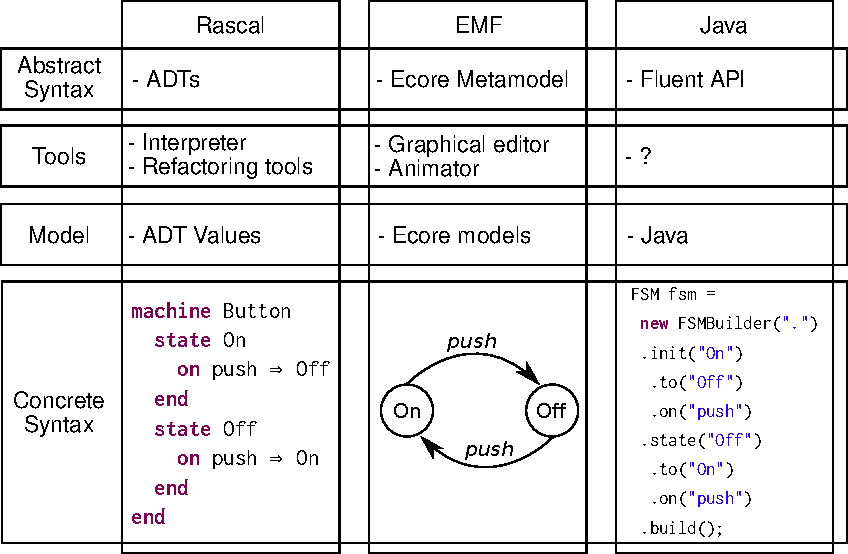
\includegraphics[width=\columnwidth]{figures/concepts-instantiated}
%	\caption{\dots}
%	\label{fig:concepts-instantiated}
%\end{figure}

\begin{figure}[bt]
	\centering
	\begin{subfigure}[b]{.3\columnwidth}
		\begin{lstlisting}[label=lst:fsm-adt, language=Rascal, numbers=none, xleftmargin=0pt, tabsize=1]
data Machine(Id uid) =
	Machine(str name,
		list[State] states,
		Ref[State] initial);

data State(Id uid) =
	State(str name,
		list[Trans] trans);

data Trans(Id uid) =
	Trans(str event,
		Ref[State] target);
		\end{lstlisting}
		\caption{Rascal ADT}
	\end{subfigure}
	\vrule
	\enskip
	\begin{subfigure}[b]{.26\columnwidth}
		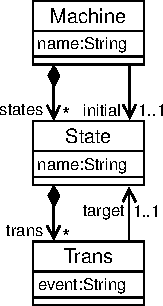
\includegraphics[width=\textwidth]{figures/fsm-mm}
		\caption{Ecore MM}
	\end{subfigure}
	\enskip
	\vrule
	\enskip
	\begin{subfigure}[b]{.35\columnwidth}
		\begin{lstlisting}[label=lst:fsm-api, language=Java, numbers=none, xleftmargin=0pt, tabsize=1]
class Fsm {
	Fsm(String name);
	State init(String name);
	State state(String name);
	Fsm end();
}
class State {
	State state(String name);
	Trans tgt(String name);
	Fsm end();
}
class Trans {
	Trans tgt(String name);
	State on(String event);
	Fsm end();
}
		\end{lstlisting}
		\caption{Java API}
	\end{subfigure}
	\caption{Three shapes of an FSM language}
\end{figure}

\subsection{Rascal}

The FSM language is defined in Rascal by the ADTs Machine, State and Trans.
A Machine has a name, contains a list of States and has a reference to an initial State.
States have a name and contains a list of Trans.
Trans is triggering an event and has a reference to an outgoing State.
The instantiation of any of theses types produce ADT values containing a unique identifier.
The containment references between ADT values are realised by lists of ADT values. But Rascal is a tree based language and there is no built in concept for simple reference.
The ADT Ref emulate this concept by containing an identifier equal to an identifier from an existing Machine,State or Trans.

\subsection{Ecore}

The same FSM language is defined by an Ecore metamodel containing the EClasses Machine, State and Trans.
Machine is the root container. It has an EAttribute ’name’, a containment EReference ’states’ typed State and a simple EReference ’initial’ typed State.
The EClass State has an EAttribute ’name’ and a containment EReference ’transitions’ typed Trans.
The EClass Trans has an EAttibutte ’event’ and a simple EReference ’target’ typed State.

\subsection{Java}

Another definition of the FSM language is done by a fluent Java API.
This shape allows to embed an Fsm model in a Java program by an expression starting with "new Fsm()" and ending with ".end()".
The API contains the classes Fsm, State and Transition.
The name of the Fsm is set by its constructor.
The reference to the initial state is expressed by the method initial taking the name of the referenced State as parameter.
The first contained States is added by method state() requiring a name as parameter.
The class State includes a method target() to add a contained Transition. It takes the name of a State as parameter to reference the outgoing State of the Transition.
By declaring the method state() too, the creation of States can be called in chain to fill the containing Fsm.
The class Transition add a method on() taking the name of an event to optionally set a triggering event on the transition.
Transition also provides the method target() to chain the creation of Transition in the containing State.

An API is fluent if it can be used in a way that looks like a program.
The FSM is represented as a sequence of method invocation.
The references are represented by argument of type String that allows the user to reference a State by its name.

As a fluent API is an embedded language, we need a mechanism to identified which range of a file is representing an FSM model.

A source of divergence with other Shapes of FSM is the encoding of the initial State.
We choose to represent a State by the method state() or by the method initial().
As the initial State is unique, we enforce its declaration as the first method invocation in the FSM. This solution solve the uniqueness but enforce the first state to be initial that it can be a source of divergence if models in other shape have a reference designating the initial state that is not in the first position. (if the order of State is part of the State Identifier)

The Java fluent API shape tends to break more easily the synchronization of their incarnations of models than the other shapes.
Indeed this shape of FSM language is an embedded language and has to rely on the host language for both the tooling and the expressiveness.
In the case of Java as host language, the validation service provided by the editor has no knowledge about the FSM language.
It makes harder for the user to detect mistakes such as typo. The FSM model can be in unnoticed dirty state and this can lead to the production of dirty Patches.
In the opposite the incarnation of the model can receive inapplicable Patches in this technological space.
For example in the Java TS, receiving a Patch telling to reference the second state of an FSM as the initial state is not possible due to the expressiveness of the API and this result in the desynchronization of the incarnation of the model.

The inconsistency of the incarnations of a model happen when one of them produce a dirty Patch or when one of them can't apply a Patch.
